% !TEX root = ../thesis.tex
\chapter{基于自适应相似性矩阵的无监督度量学习}
\section{引言}
数据在数据空间中的空间分布学习一直是一个困难的问题。经验上,数据往往分布在高维空间的一个低维流形上,而不是完全随机分布。这导致了不同标签的数据之间可能有较近的欧氏距离。这种分布特性会对基于传统欧氏距离度量的分类或聚类算法的效果产生影响。一个较好的选择是构建一个能够保持数据对之间局部近邻结构的低维映射。

谱聚类方法是一类在基于矩阵特征分解的聚类方法,该类方法在很多具有挑战性的真实世界数据集上表现出了非常优异的性能。在最近几十年间,一系列经典的谱聚类方法被提出,例如:多维标度法(Multidimensional Scaling,MDS)\cite{cox2000multidimensional},局部线性嵌入(Local Linear Embedding,LLE)\cite{roweis2000nonlinear},等距特征映射(Isomap)\cite{tenenbaum2000global},拉普拉斯特征映射(Laplacian Eigenmaps)  \cite{belkin2001laplacian}和变种的谱聚类\cite{ng2002spectral}. 上述提到的谱聚类算法有三点不足之处。第一,这些谱聚类算法只提供了训练数据的嵌入映射,对样本外数据(out-of-sample)的计算比较困难。第二,这些算法的复杂度依赖于数据点数量,相对比较耗时,可扩展性不强。第三,谱聚类算法的稳定性高度依赖于相似性图(affinity graph)的鲁棒性。

为缓解上述谱聚类中存在的问题,大量重要的研究进展被提出\cite{bengio2004out,niyogi2004locality,fowlkes2004spectral,yan2009fast,chen2011large,pavan2007dominant,premachandran2013consensus,zhu2014constructing,nie2014clustering}。局部保持投影(Locality Preserving Projections, LPP)\cite{niyogi2004locality}引入了一种由拉普拉斯特征映射得到的线性投影方法。他们的工作提供了一种嵌入映射的线性近似,该线性近似可以减少计算复杂度并可以简单的实现样本外数据的扩展。线性嵌入提供了一种度量学习角度下的谱聚类方法。文献\parencite{nie2014clustering}提出了自适应近邻投影聚类(Projected Clustering with Adaptive Neighbors,PCAN)算法,该算法将点对之间的相似性作为一个额外的待求解变量并且通过对图拉普拉斯(graph Laplacian)矩阵的秩设置惩罚项以限制相似性矩阵的连通区数量。基于这个框架,PCAN算法交替地更新相似性矩阵和投影。经验上,流形嵌入方法的效果依赖于相似性矩阵的鲁棒性。图\ref{fig2:affMat}给出了MNIST数据集\cite{lecun1998gradient}的子集在理想情况下及不同近邻数量下的热力核相似性矩阵。从图中可看出广泛使用的$k$近邻($k$ nearest neighborhood,$k$-NN)热力核中存在大量的噪声。虽然一些相似性学习的方法已经被提出,选择合适的相似性矩阵的问题依然有待解决。

\begin{figure}[!hbtp]
	\centering
	\bisubcaptionbox{理想的相似性矩阵}%
					{Ideal affinity matrix}
					[0.3\textwidth]{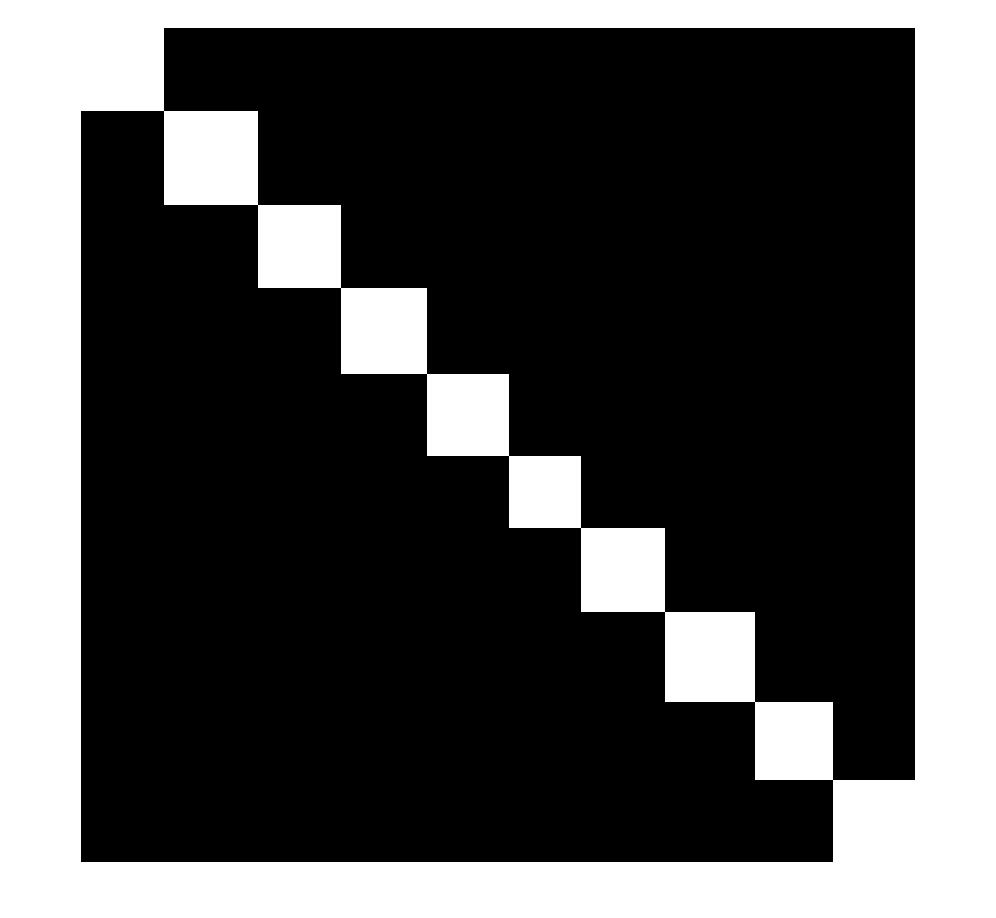
\includegraphics[width=0.3\textwidth]{chap2/k1.jpg}}
	\hspace{1em}
	\bisubcaptionbox{$k=100$下的热力核相似性矩阵}%
					{Affinity matrix of heat kernel with $k=100$}
					[0.3\textwidth]{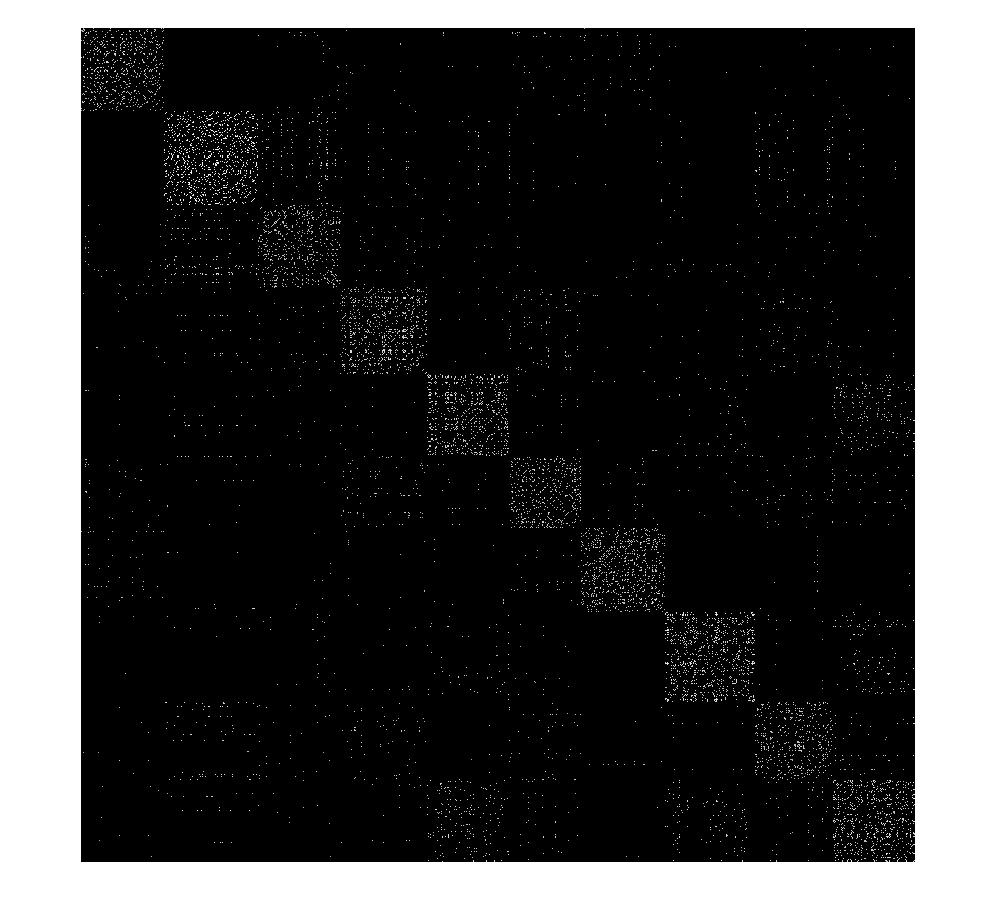
\includegraphics[width=0.3\textwidth]{chap2/k100.jpg}}
	\hspace{1em}
	\bisubcaptionbox{$k=1000$下的热力核相似性矩阵}%
					{Affinity matrix of heat kernel with $k=1000$}%
					[0.3\textwidth]{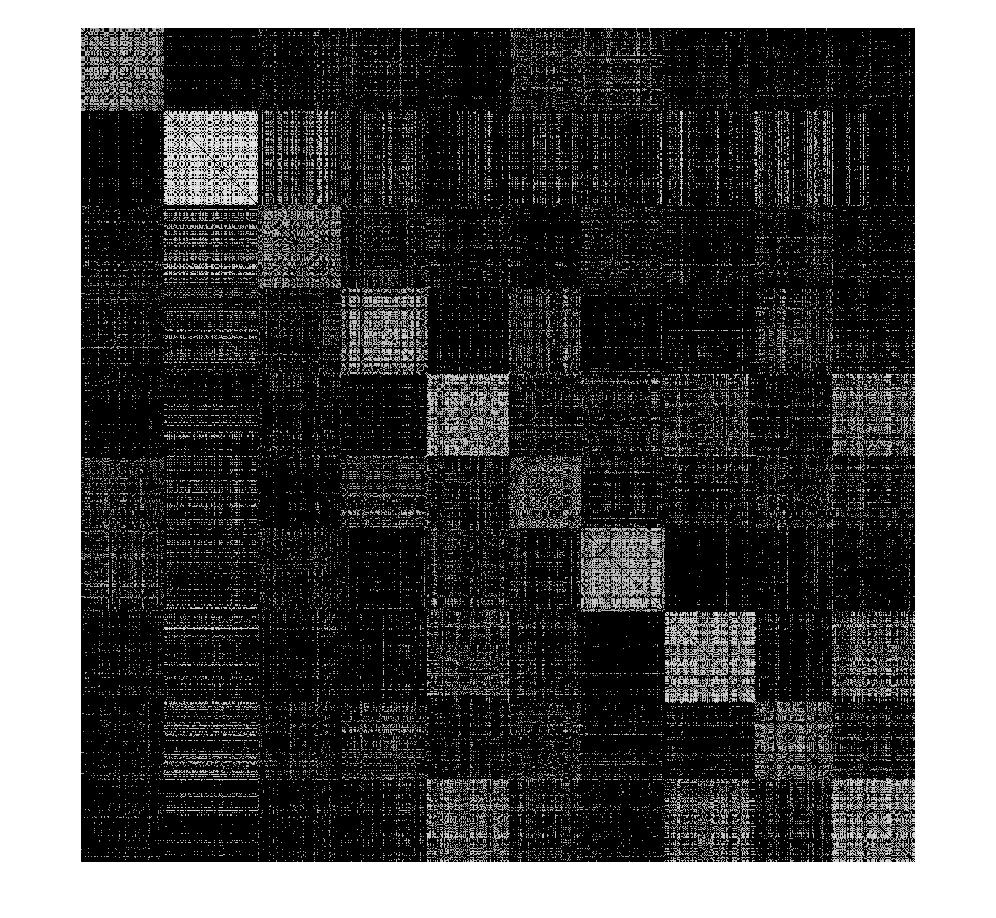
\includegraphics[width=0.3\textwidth]{chap2/k1000.jpg}}
	\bicaption{MNIST子集在理想情况及不同近邻数量$k$下的相似性矩阵。}
			  {Ideal affinity matrix and affinity matrices with different neighborhood size $k$ on a subset of MNIST}
  	\label{fig2:affMat}
\end{figure}

本章所提出的方法的目标在于,针对谱聚类的线性近似,在最小的时间消耗下,提取更具有自适应性的相似性信息。这类信息将会更多的考虑局部性保持(locality preserving)这个优化目标,而不仅仅是图像间的距离。受到可扩展谱聚类和数据相似性学习方向上的研究成果\cite{chen2011large,nie2014clustering}的启发,本章提出了一个新颖的自适应相似性矩阵(Adaptive Affinity Matrix,AdaAM)方法。该方法的相似性矩阵相对稠密并可以同时捕捉到全局及局部信息。特别地,AdaAM将相似性矩阵分解成两个相同的低秩矩阵的乘积。作为文献\parencite{ng2002spectral}中描述的理想情况,如果我们假设同一个类内的点对相似性极为相似,则相似性矩阵可能会形成一个低秩矩阵。本算法采用与谱聚类方法相似的优化方法对分解后的矩阵进行优化求解。优化得到的相似性图作为最终结果前的中间态相似性矩阵。通过合并基于热力核获得的$k$-NN相似性图和中间态相似性矩阵,AdaAM采用朴素的谱聚类求解方法计算出一个最终的自适应相似性矩阵。我们将LPP方法作用于此特定的相似性矩阵上进行数据投影,以获得一个用于聚类的距离度量。

在本章中,我们将通过在图像数据集上的聚类实验展示所提出方法的有效性和高效性。第 \ref{sec2:Exp}节通过对本章提出的算法和基于$k$-NN的拉普拉斯特征映\cite{belkin2001laplacian}以及其他最先进方法进行对比展现了AdaAM方法在具有挑战性的数据集上的聚类效果具有明显优势。


\section{自适应相似性矩阵}
在本节中,我们首先对本节采用的数学符号进行说明,其次介绍中间态相似性矩阵的计算方法,然后描述最终自适应相似性矩阵的获取方式,最后对算法流程中的稀疏化策略进行介绍。
\subsection{符号说明}
在本章中,我们以大写英文或希腊字母代表矩阵,小写字母代表向量。所有元素全部为$1$的向量用$\bf{1}$表示。$H$表示中心化矩阵(Centering Matrix),其定义为:$H = I-\frac{1}{n}\bf{1}\bf{1}^T$。原始数据矩阵以$X \in \mathbb{R}^{n\times d}$表示,其中$n$为数据点的数量,$d$为数据维数。本章中将假设数据矩阵$X$为零均值标准化矩阵,即$X = HX$。符号$x_i$表示数据矩阵$X$中的第$i$个数据点向量。我们用$A$表示线性投影,相应的距离度量矩阵表示为$M = A^TA$。因此,在该度量矩阵下的距离定义为$dis_m(x_i, x_j) = (x_i - x_j)^TM(x_i - x_j)$。我们将$k$-NN热力核矩阵表示为$W \in \mathbb{R}^{n \times n}$:
\begin{equation}
	w_{ij} = \begin{cases} \mathrm{exp}(-\frac{\|x_i-x_j\|_{2}}{t}), \; &x_i\in\mathcal{N}_k(x_j)\;\mathrm{or}\; x_j\in\mathcal{N}_k(x_i);\\
		0, &\mathrm{otherwise.}\end{cases}          
\end{equation}
此处,$\mathcal{N}_k(x)$表示数据点$x$的 $k$ 个最近邻的集合。相应的拉普拉斯矩阵表示为$L=D-W$,其中$D$为对角权重矩阵:$d_{ii} = \sum_j w_{ij}$。我们对中间态增量矩阵及最终自适应相似性矩阵都采用$\Delta$表示,相应的对角权重矩阵和拉普拉斯矩阵分别表示为$D_\Delta$和$L_\Delta = D_\Delta-\Delta$。

\section{中间态相似性矩阵}
我们将提出的AdaAM算法分为两个部分,分别是中间态相似性矩阵和最终自适应相似性矩阵。本节将对其中的中间态相似性矩阵部分的生成进行介绍。对于第$i$个数据点$x_i$,我们使用相似度$\delta_{ij}$对任意的数据点$x_i$和数据点$x_j$进行连接。由于希望任意两个数据点之间较近的欧氏距离能导致较大的数据点相似度,我们的目标为通过选择最优的相似度$\delta_{ij}$在特定合适的约束下最小化下述的目标函数,
\begin{equation}
	\mathop{\mathrm{min}} \sum_{i,j}^{n} \|x_i-x_j\|_2^2\;\delta_{ij},
\end{equation}
在这里,$\delta_{ij}$表示中间态相似性矩阵$\Delta$中第$ij$个元素。

不同于PCAN算法\cite{nie2014clustering},我们基于图拉普拉斯对该目标函数公式在其约束条件下进行变形,
\begin{equation}
	\mathop{\mathrm{min}}\; tr(X^TL_\Delta X).
	\label{eq2:Delta}
\end{equation}

由于在通常情况下图拉普拉斯为半正定矩阵,因此一个直接又看似可行的思路是将拉普拉斯矩阵分解为两个相同矩阵的乘积。在下文中我们将论述该思路不适用于我们的计算框架。

我们采用$U\in \mathbb{R}^{n\times s}$ 表示一个列正交矩阵,以满足$U^TU = I$,则我们可以假设
\begin{equation}
	L_\Delta = UU^T.
\end{equation}
在对原优化问题进行约束松弛的情况下,我们最终需要求解问题为:
\begin{equation}
	\begin{split}
		&U = \mathop{\mathrm{arg\;min}}_{U^TU=I}\; tr(X^TUU^TX) \\
		&\Rightarrow U = \mathop{\mathrm{arg\;min}}_{U^TU=I} \;tr(U^TXX^TU)
	\end{split}
	\label{eq2:simpEigmap}
\end{equation}

如果我们假设矩阵$X$的乘积为矩阵$K$,即$K = XX^T$,则公式(\ref{eq2:simpEigmap})所得为一个简单形式的拉普拉斯特征映射\cite{belkin2001laplacian}。
由此,该优化问题可以通过选择矩阵$K$的多个最小特征值所对应的特征向量形成矩阵进行求解。但是,由于$K$为一个低秩矩阵,一般情况下满足条件$d\ll n$,$K$可以最小化公式(\ref{eq2:simpEigmap})中目标函数的特征向量都存在于数据矩阵$X$的零空间中。
因此,上述问题的最优解不唯一。受LSC(Landmark-based Spectral Clustering)算法\cite{chen2011large}启发,我们将相似性矩阵假设为一个半正定矩阵。不同于对拉普拉斯矩阵进行分解,我们将半正定的相似性矩阵分解为列正交矩阵 $P\in \mathbb{R}^{n\times t}$及其转置矩阵$P^T$的乘积,其中 $t$ 为预期下的矩阵$\Delta$的秩。

由此,我们可以将公式(\ref{eq2:Delta})改写为
\begin{equation}
	% 	\begin{split}
	% 		&\mathop{\mathrm{min}}_{P^TP=I} tr(X^T(D_\Delta-PP^T)X) \\
	% 		&\Rightarrow 
	\mathop{\mathrm{min}}_{P^TP=I} tr(X^TD_\Delta X)+tr(X^T(-PP^T)X),
	% 	\end{split}
	\label{eq2:XLX}
\end{equation}
此处,

\section{实验结果}
\label{sec2:Exp}